% !TeX root = ../thuthesis-example.tex

\chapter{系统实现}
在第3章和第4章中,本文设计了全局对称模式挖掘算法和
分段对称模式挖掘算法两种不同的算法,并根据不同应用场景
的特殊约束将其扩展到了流式数据和变长模式中。
通过第5章中的实验发现,两种对称模式挖掘算法不仅具有最好的
挖掘效果,而且在时间效率上也远远超过基于动态时间扭曲的算法。
接下来,本章通过将这两种算法集成到IoTDB的数据质量工具库
IoTDB-Quality中,帮助用户挖掘时间序列中蕴含的对称模式信息,
并方便在此基础上执行更复杂的数据分析工作。

\section{总体介绍}
IoTDB-Quality基于IoTDB用户自定义函数(UDF),
实现了一系列关于数据质量和分析的函数,
包括数据画像、数据质量评估与修复、数据匹配和模式发现等,
有效满足了工业领域对数据挖掘的需求。
当对一个长时间序列进行预测和异常检测时,
如果能提前识别时间序列中蕴含的模式,将能够对
时间序列未来的发展变化具有一个清晰明确的预期,
为用户提供预测或异常修复的有效参考,从而提高时间序列数据的质量。

\begin{figure}
    \centering
    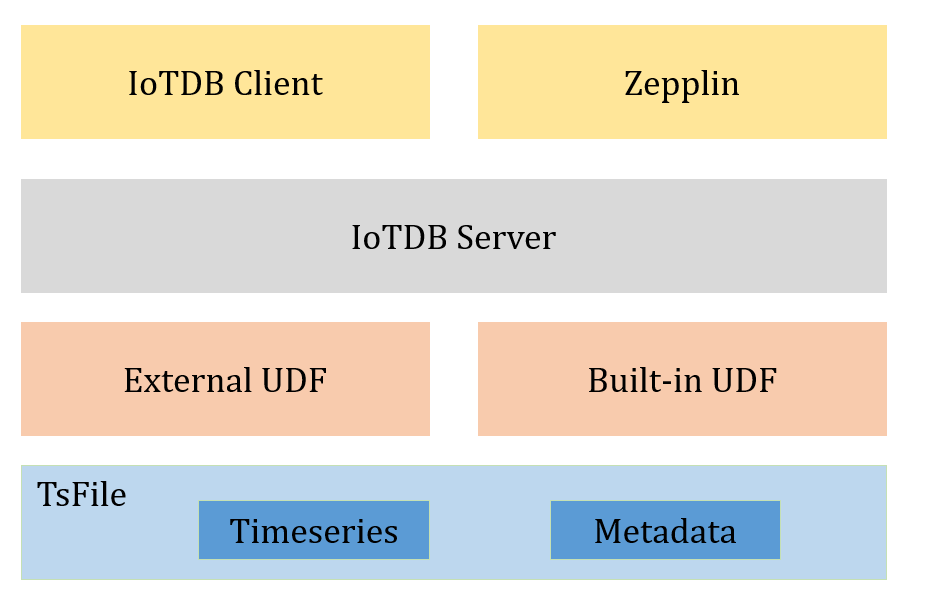
\includegraphics[width=0.66\linewidth]{udf-structure.PNG}
    \caption{基于IoTDB实现的对称模式挖掘算法架构图}
    \label{fig:symmetry_structure}
\end{figure}

IoTDB为用户提供了一套成熟的函数管理和执行框架,本文的算法实现即基于
此框架。如图~\ref{fig:symmetry_structure}所示,由于IoTDB的底层存储结构
TsFile为列式存储,首先通过Transformer层将列式存储的数据根据时间戳
归并到一个RowRecord中,然后由本文设计实现的全局和分段算法
根据固定的数据访问策略读取数据并完成对称模式的挖掘,将挖掘结果返回给
IoTDB并由命令行客户端或Apache UI工具Zepplin展示挖掘结果。

\section{全局对称模式挖掘算法实现}
IoTDB为用户提供了一个用于时间序列数据分析的自定义模板函数接口UDTF
(User Defined Timeseries Generating Function),
该模板支持多条时间序列和多个参数的输入,最终会输出一条时间序列数据
表示函数计算的结果。对于全局对称模式算法而言,根据第3.1章的计算流程,
只需要输入一条完整的时间序列数据用于挖掘对称模式,具体的
全局对称性度量和对称度阈值确定都可以在函数处理中由算法确定。
在具体实现中,为方便用户使用,本算法提供了阈值(threshold)参数,
可以由领域专家自行指定对称度阈值,若不指定,则采用对称度阈值确定算法进行计算。
本算法用到了UDTF中定义的四个接口,具体实现方式如下所示:
\begin{itemize}
\item validate:验证算法的参数是否输入正确,threshold代表时间序列的
      对称度,一定是正数。如果不输入,则代表使用自定义的对称度阈值确定算法。
\item beforeStart:指定滑动窗口的数据访问策略并执行算法的初始化。由于
      全局对称模式挖掘算法是对时间序列整体计算对称性,因此,设定时间序列的
      窗口大小为无穷大以将全部数据加载到算法中。
\item transform:执行全局算法以挖掘对称模式,具体步骤如下所示:
    \begin{enumerate}
        \item 对长度小于2的时间子序列的对称度进行初始化计算。
        \item 按照长度由小到大的顺序推导并计算每一段时间子序列的对称度,并将结果
              保存在预定义的数据结构中。
        \item 根据时间序列的数据特征进行差分计算,得到对称度阈值。
        \item 由计算得到的全局对称度和对称度阈值判定输入时间序列是否属于对称模式。
    \end{enumerate}
\item terminate:将全局时间序列是否具有对称性的判定结果输出到collector中。
    
\end{itemize}

\section{分段对称模式挖掘算法实现}
分段对称模式挖掘算法的处理过程和全局对称模式挖掘算法有所不同,
根据3.2章的计算流程,除了需要输入一条完整的时间序列数据,
还需要输入分段对称模式窗口大小,以及由用户自定义的对称度阈值。
对于算法的输出,由于现在的UDTF并不支持分组的结果展示,
将所有的对称模式拼接到一起展示又扰乱了展示结果。
因此,在本算法的实现中,对于每一个分段对称模式,算法只输出
对称模式的起始时间点和其对称度信息,具体的计算流程如下所示:
\begin{enumerate}
    \item 首先,IoTDB通过序列读取器读取时间序列数据,
    由于需要根据全部子序列的对称度特征进行阈值划分,
    所以要把所有的数据全部加载到内存中,保存在算法的
    自定义数据结构中。
    \item 然后,在transformer函数中定义动态规划
    状态信息,按照区间由小到大的顺序计算所有长度小于w的
    子序列的对称度。需要注意的是,由于输出时需要明确分段模式
    的起始时间,所以需要将RowWindow中每个时间子序列的
    起始点时间信息保存下来。
    \item 对transformer函数中保存的数据值进行差分计算,求得
    相邻点距离的平均值。再采用流式算法计算子序列对称度的方差,
    根据方差之和最大原则寻找自然断点。利用上述两个阈值候选的最小值
    求得分段对称模式的真实阈值。
    \item 根据贪心策略计算出数量最多的对称模式,并将结果循环输出到
    collector中。
\end{enumerate}

为加速UDF的计算速度,在算法的实现中放弃使用了语言自带的集合类,
因为集合类会对基础类型进行包装,在拆箱和装箱的过程中会降低算法的性能。
在算法的实现过程中,本文对用到的每种数据结构都进行了重新实现,
提高了算法的效率。

\section{算法查询展示}

在实现了对称模式挖掘的算法逻辑之后,用户可以使用两种方式
执行算法并对结果进行查询。一种是利用IoTDB-Client命令行,
另一种是在Apache Zepplin上通过前端UI进行查询。
在命令行上,用户登录客户端之后,直接输入调用UDF函数的SQL语句
进行查询,查询结果如图~\ref{fig:iotdb_client_symptn}所示。
直接使用select语句就可以查询全局和分段对称模式的挖掘结果。
使用IoTDB Client命令行进行查询的好处是查询便捷,
直接登陆客户端即可查询,不需要重新部署其他工具。
但是,在命令行查询的结果只能通过表格的方式
进行展示,不方便直观的观察查询结果。仅通过在命令行中观察,
用户无法区分~\ref{fig:gsymptn_input}所示的查询数据是否
具有对称性,因而更无法对查询结果的正确性进行判断。
基于此,在IoTDB-Client上进行查询只适用于开发中的结果验证,
不适合商业化用户使用。因此,需要配置部署一个直观的前端查询方式。
\begin{figure}
    \centering
    \subcaptionbox{数据集\label{fig:gsymptn_input}}
    {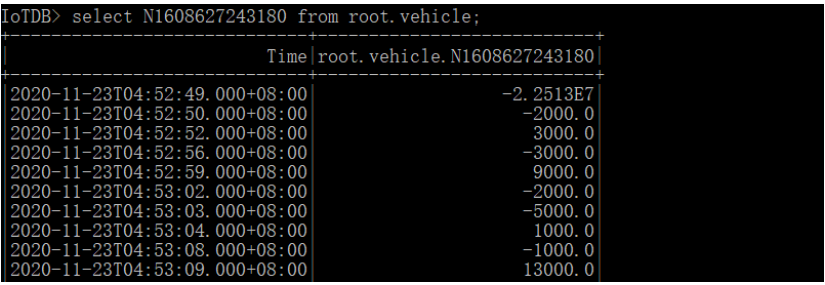
\includegraphics[width=0.86\linewidth]{gsymptn_input.PNG}}
    \subcaptionbox{查询结果\label{fig:gsymptn_output}}
    {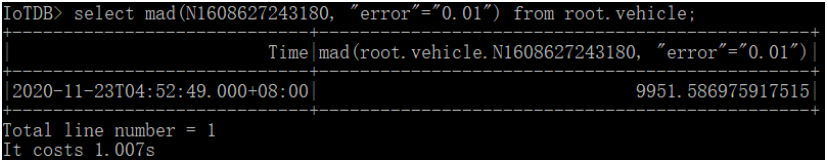
\includegraphics[width=0.86\linewidth]{gsymptn_output.PNG}}
    \caption{在IoTDB-Client运行对称模式挖掘算法的结果查询展示}
    \label{fig:iotdb_client_symptn}
\end{figure}

Apache Zepplin是一个是一个基于网页的交互式数据分析系统。
用户可以通过Zeppelin连接IoTDB数据源并使用SQL进行交互式查询操作。
图~\ref{fig:iotdb_zepplin_symptn}中展示了在Zepplin上进行
对称模式挖掘结果计算并查询的方式,图中上半部分是在Gun point
数据集中挖掘判定全局对称模式。利用Zepplin自带的散点图和折线图
用户可以方便的观察出Gun point数据集中的时间序列具有全局对称性。
最终的查询结果也印证了直观的判断。图中下半部分是在挖掘机工况
数据集上挖掘分段对称模式,在Zepplin的输入框中直接输入select语句
就可以像IoTDB-Client命令行一样执行查询,通过前端的各类统计图
可以方便的观察到分段对称模式的数量信息,通过与分段算法
的结果进行对比,可以验证分段对称模式挖掘算法的效果。

\begin{figure}
    \centering
    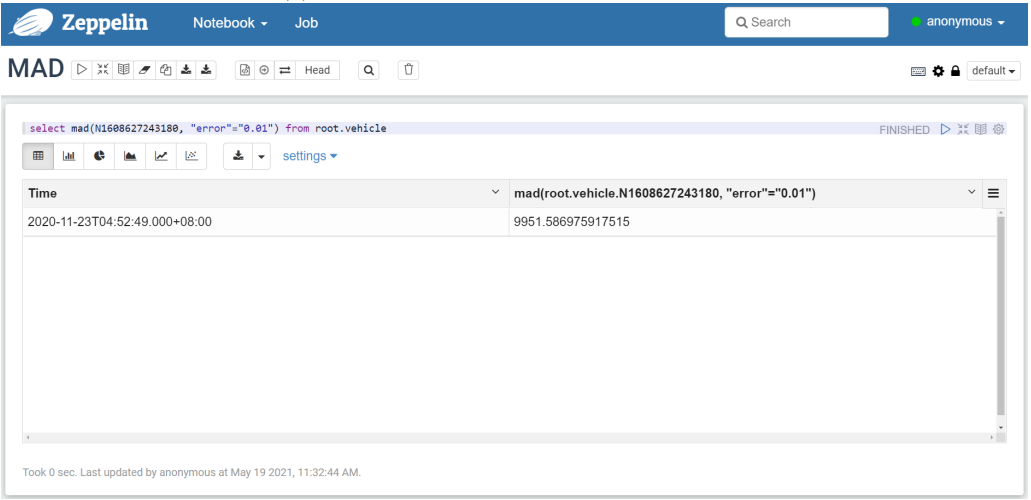
\includegraphics[width=0.86\linewidth]{gsymptn_zepplin.png}
    \caption{在Apache zepplin运行对称模式挖掘算法的结果查询展示}
    \label{fig:iotdb_zepplin_symptn}
\end{figure}


\section{本章小结}
本章主要介绍了根据IoTDB提供的用户自定义函数模板接口,
全局对称模式挖掘算法和分段对称模式挖掘算法的实现方式,
并通过在IoTDB Server上进行部署,使用IoTDB Client和
Apache Zepplin两种方式进行函数调用计算和结果查询。
通过基于IoTDB实现这两种算法,弥补了IoTDB Quality挖掘对称模式
的功能缺失,在帮助用户得到蕴含在时间序列中对称特征的同时,
便于发现违反模式规律的异常点并进行检测和修复。